


% Please add the following required packages to your document preamble:
% \usepackage[normalem]{ulem}
% \useunder{\uline}{\ul}{}

\begin{figure}[htp]
    \centering
    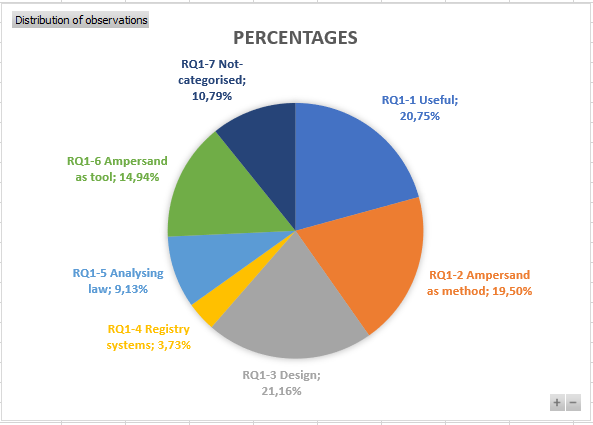
\includegraphics[width=0.7\textwidth]{docs/AF-SE/00_common/04_images/content_analysis.PNG}
    \caption{Content observations Distribution}
    \label{fig:content distribution}
\end{figure}

\def\head{\textbf{RQ1-1, Category:Useful, Reference to observation/interview}}
\begin{xltabular}{\textwidth}{|X|}
\caption{List of observations \head} \\ \hline 
\multicolumn{1}{|l|}{\head}  \\ \hline 
\endfirsthead
{{\bfseries \tablename\ \thetable{} -- continued from previous page}} \\
\hline 
\multicolumn{1}{|l|}{\head}  \\ \hline 
\endhead
\hline \multicolumn{1}{|r|}{{Continued on next page}} \\ \hline
\endfoot \hline \hline
\endlastfoot
-	rq1-11 Implementation in \A{Docker} with RAP creates new directories all the time.
\\-	rq1-13:17-10: The setup of \A{Ampersand} in local environment is specific and not self-explanatory.
\\-	rq1-17 Applying a rule requires a lot of patience and practice.
\\-	rq1-18 Can not find an example on the internet, only in the repo of \A{Ampersand} itself.
\\-	rq1-39:3-10: Do not forget to create delete rules in addition to append and edit rules in the {rule}\textbf{s} in the context of the \A{Lifecycle} approach.
\\-	rq1-42:19-10: Immediately add the description when recording a {concept} and \A{relation}.
\\-	rq1-42:21-10: It is easy to deviate from the legal texts.
\\-	rq1-45:24-10: Overview within a \A{Ampersand}script is difficult to maintain and obtain.
\\-	rq1-46:24-10: There is no find able relationship between the \A{relation} and the {concept} in the script.
\\-	rq1-47:27-10: Detecting a bug.
\\-	rq1-60:9-11: The process of writing a \A{Ampersand} script is not without practice.
\\-	rq1-62:10-11: There has be the \A{architecture} link between the {law core} and the {register core}
\\-	rq1-63:10-11: Ampersand is \A{flexible} by extension concepts and relationships.
\\-	rq1-7:10-11: Each \A{relation} is part of a record structure.
\\-	rq1-70:14-11: Postman works with api/v1/resource, e.g. GET \url{localhost/api/v1/resource/Person/P001/Person}, retrieves that of an existing person.
\\-	rq1-73:14-11: Ampersand can be used from other applications through \A{api}'s, but the return values are next to the requested information also messages and not message codes.
\\-	rq1-96:30-12: Skill in scripting within \A{Ampersand} is quickly lost if you don't do this frequently.
\\-	rq1-97:30-12: By puzzling with Ampersand people quickly forget to make correct \A{documentation}.
\\-	rq2-12:19-10: TOT has the property that this must be entered in the \A{interface} because otherwise the data will not be saved.
\\-	rq2-16:19-10/11-11: Ampersand has a hard time determining a period.
\\-	rq2-18:16-11: Good to realize that the {meaning} you write down also ends up in the \A{Conceptual analysis}.
\\-	rq3-7 Adding \A{documentation} with the correct description to a concept and relation is not so easy.
\\-	rq4-5 Postman used for \A{api} link with Ampersand.
\\-	rq4-7 What happens if \A{Ampersand} is implemented and there are changes in the structure (normal for software)
\\-	rq4-8:22-11: The team behind \A{Ampersand} is very dedicated.
\\-	 rq1-8:14-11: No swagger is created for the \A{api}
\\-	rq1-46:24-10: There is no find able relationship between the {relation} and the \A{concept} in the script.
\\-	 rq1-6:21-10/30-10: \A{Docker} is also another thing to learn.
\\-	 rq1-17 Applying a \A{rule}\textbf{s} takes a lot of patience and practice.
\\-	 rq2-4:30-9: Which agreements must be made regarding the structure of the descriptions for \A{Conceptual analysis}.
\\-	 rq3-16:24-10: For the Netherlands, we have a country table from the RvIG.
\\-	 rq4-2 The \A{api} link works fine, but entire messages return.
\\-	Ampersand can be interesting, because it will be able to clear conflicting matters from the law.
\\-	The registry core, an architecture model of CIBG, uses shared concepts
\\-	In addition, the implementation must be such that the effective dates of the specific amendments to the law are also taken into account.
\\-	Ampersand's possible positioning is to use it as an interpreter of legislation and regulations
\\-	Ampersand has APIs and that is interesting to be able to link with
\\-	When maintenance takes place on the model, how do we get from one model to another
\\-	Ampersand's approach is in line with the \acrlong{rk}, but not at the implementation level.
\\-	An addition of Ampersand is that a prototype is made that can also be tested. 
\\-	A draft of the conceptual analysis is available and this is experienced as trusted by the lawyer. 
\\-	Going through the law should be a first step for the conceptual analysis.
\\-	The prototype shown is not easy for the user to understand.
\\-	Ampersand's deployment could be applied to new tasks.
\\-	For use, the question is how quickly a base is set up
\\-	Ampersand method is a way of writing things down
\\-	How is the maintenance of the system? A new model is always made with the help of Ampersand.
\\-	The learning curve doesn't seem that big. 
\\-	The question is whether the system will only work for simple registers or whether we can also use it to tackle complex registers.
\\-	A follow-up study could be to make a comparison between a system built traditionally and a system built on the Ampersand method. 

\end{xltabular}

\def\head{\textbf{RQ1-2, Category:Ampersand as method, Reference to observation/interview}}
\begin{xltabular}{\textwidth}{|X|}
\caption{List of observations \head} \\ \hline 
\multicolumn{1}{|l|}{\head}  \\ \hline 
\endfirsthead
{{\bfseries \tablename\ \thetable{} -- continued from previous page}} \\
\hline 
\multicolumn{1}{|l|}{\head}  \\ \hline 
\endhead
\hline \multicolumn{1}{|r|}{{Continued on next page}} \\ \hline
\endfoot \hline \hline
\endlastfoot
-	rq1-21:7-11: TOT is usually overcome by a tot-rule, it turns out that a TOT causes something to be saved when entered, while a tot-rule allows a save to occur while the notification remains open to stand.	\\
-	rq1-25:12-9: First make \A{overview} of all laws and regulations	\\
-	rq1-3 Created a separate excel to write out and discover the \A{multiplicity} of the relations.	\\
-	rq1-30:12-9: Defining the meaning and definition of the \A{concept} is free.	\\
-	rq1-33:14-9: The use of \A{pattern}s within Ampersand is important.	\\
-	rq1-38:3-10: Should the subsystems be mapped in advance.	\\
-	rq1-4 Automatically executed \A{rule} are easy to describe, but implementation here also takes a lot of patience and trying.	\\
-	rq1-42:19-10: Immediately add the description when recording a {concept} and \A{relation}.	\\
-	rq1-46:24-10: There is no find able relationship between the \A{relation} and the {concept} in the script.	\\
-	rq1-51:2-11: Discussing the \A{Conceptual analysis} should be done theme by theme.	\\
-	rq1-55:2-11: At the \A{rule} it is necessary to add a ROLE with a MAINTAINS, otherwise the rule will not work.	\\
-	rq1-57-1:7-11: Using Ampersand for \A{validation}.	\\
-	rq1-61:9-11: There should be a check on the draft date of birth(\A{rule}), so that someone must be at least 18.	\\
-	rq1-63:10-11: Ampersand is \A{flexible} by extension concepts and relationships.	\\
-	rq1-67:11-11: If there is an automatic \A{rule}, should there still be a validation rule on it?	\\
-	rq1-7:10-11: Each \A{relation} is part of a record structure.	\\
-	rq1-80:20-11: A consistent naming of a \A{concept} is necessary.	\\
-	rq1-84:30-11: A \A{concept} is immutable.	\\
-	rq1-89:7-12: Items named as common \A{concept}s.	\\
-	rq1-90:14-12: Collection model of regulations than by means of \A{include}s keep it small and therefore clear.	\\
-	rq1-91:14-12: A {concept} and a \A{relation} can be defined several times within your own patterns.	\\
-	rq2-10:19-10: The naming of a \A{relation} is usually assigned to the TRG attribute of the set.	\\
-	rq2-11:19-10: An \A{relation} that is univalent is a function.	\\
-	rq2-12:19-10: TOT has the property that this must be entered in the \A{interface} because otherwise the data will not be saved.	\\
-	rq2-12:19-10: TOT has the property that this must be entered in the {interface} because otherwise the data will not be saved.	\\
-	rq2-13:19-10: What applies to \A{multiplicity} TOT, also applies to SUR. 	\\
-	rq2-4:30-9: Which agreements must be made regarding the structure of the descriptions for \A{Conceptual analysis}.	\\
-	rq2-5:2-10: Making the \A{multiplicity} explicit.	\\
-	rq2-8:7-10/10-10: Date of birth must be formatted as date.	\\
-	rq4-1 Ampersand cannot calculate.	\\
-	rq4-2 The \A{api} link works fine, but entire messages return	\\
-	rq4-7 What happens if \A{Ampersand} is implemented and there are changes in the structure (normal for software)	\\
-	 rq2-19:16-11: \A{Ampersand} returns constraints and no executable	\\
-	 rq2-14:19-10: The role gives control to the user.	\\
-	 rq2-2 Only UNI, TOT, INJ and SUR are used.	\\
-	The assumption made by the interviewee that Ampersand is a tool that performs an interpretation on the law itself, is not correct. 	\\
-	The registry core, an architecture model of CIBG, uses shared concepts.	\\
-	The danger of using legislation and regulations is that there is a possible incomplete picture of the concepts.	\\
-	Ampersand's possible positioning is to use it as an interpreter of legislation and regulations. 	\\
-	Ampersand relies on facts and not on processes.	\\
-	An addition of Ampersand is that a prototype is made that can also be tested. 	\\
-	Going through the law should be a first step for the conceptual analysis.	\\
-	For use, the question is how quickly a base is set up	\\
-	How is the maintenance of the system? A new model is always made with the help of Ampersand.	\\
-	The learning curve doesn't seem that big	\\
-	The Ampersand approach is different from most products	\\
-	One could also only use the output of the analysis to build a system	\\
\end{xltabular}


\def\head{\textbf{RQ1-3, Category:Design, Reference to observation/interview}}
\begin{xltabular}{\textwidth}{|X|}
\caption{List of observations \head} \\ \hline 
\multicolumn{1}{|l|}{\head}  \\ \hline 
\endfirsthead
{{\bfseries \tablename\ \thetable{} -- continued from previous page}} \\
\hline 
\multicolumn{1}{|l|}{\head}  \\ \hline 
\endhead
\hline \multicolumn{1}{|r|}{{Continued on next page}} \\ \hline
\endfoot \hline \hline
\endlastfoot
-	rq1-1 Formatting in Ampersand (\A{pattern}s) has consequences for the {Conceptual analysis}.	\\
-	rq1-36:3-10: What about \A{prototype} test scenarios.	\\
-	rq1-39:3-10: Do not forget to create delete rules in addition to append and edit rules in the \A{rule}\textbf{s} in the context of the \A{Lifecycle} approach.	\\
-	rq1-4 Automatically executed \A{rule} are easy to describe, but implementation here also takes a lot of patience and trying.	\\
-	rq1-42:19-10: Immediately add the description when recording a \A{concept} and {relation}.	\\
-	rq1-42:21-10: It is easy to deviate from the legal texts.	\\
-	rq1-58:8-11: Per \A{interface} max 1 \A{multiplicity}, otherwise you won't get data stored.	\\
-	rq1-58:8-11: Per \A{interface} max 1 {multiplicity}, otherwise you won't get data stored.	\\
-	rq1-59:9-11: Many messages remain open if not all \A{rule}s are met.	\\
-	rq1-61:9-11: There should be a check on the draft date of birth(\A{rule}), so that someone must be at least 18.	\\
-	rq1-63:10-11: Ampersand is \A{flexible} by extension concepts and relationships.	\\
-	rq1-67:11-11: If there is an automatic \A{rule}, should there still be a validation rule on it?	\\
-	rq1-69:14-11: Postman\footnote{\url{https://www.postman.com/product/what-is-postman/}} application installed and works with the \A{prototype}.	\\
-	rq1-7:10-11: Each \A{relation} is part of a record structure.	\\
-	rq1-71:14-11/16-11: The \A{interface} also belongs to the design and not just to the prototype.	\\
-	rq1-75:20-11: Some more experimentation with the \A{documentation} in the prototype.	\\
-	rq1-78:20-11: The \A{documentation} generated in HTML loaded in firefox and no PNG's are visible.	\\
-	rq1-91:14-12: A {concept} and a \A{relation} can be defined several times within your own patterns.	\\
-	rq1-92:14-12: Basically trying to create its own container per \A{register}.	\\
-	rq1-93:19-12/21-12: Implementation choice for separate \A{register}s has an impact on the whole.	\\
-	rq1-95:29-12: The format of a \A{concept} big number is not included in the law	\\
-	rq2-10:19-10: The naming of a \A{relation} is usually assigned to the TRG attribute of the set.	\\
-	rq2-14:19-10: The role gives control to the user.	\\
-	rq2-15:19-10: In the \A{interface} a FOR can also be used.	\\
-	rq2-15:19-10: In the {interface} a FOR can also be used.	\\
-	rq2-17:10-11: A dutch person has an \A{concept} address that must conform to the BRP format (should be a standard building block for it!).	\\
-	rq2-18:16-11: Good to realize that the \A{meaning} you write down also ends up in the {Conceptual analysis}.	\\
-	rq2-9:7-10: Subscription time is added automatically.	\\
-	rq3-10:12-10: Formatting of the name is not stated literally in the \A{law}, but must conform to BRP standards.	\\
-	RQ3-11:12-10: Matters such as authorization decisions that allow an information system to retrieve BRP data are not found in the \A{law}.	\\
-	rq3-8:19-9: The law states that there are multiple registers.	\\
-	rq4-2 The \A{api} link works fine, but entire messages return.	\\
-	rq4-3 Embedding in \A{architecture}	\\
-	rq4-7 What happens if \A{Ampersand} is implemented and there are changes in the structure (normal for software)	\\
-	rq1-1 Formatting in Ampersand ({pattern}s) has consequences for the \A{Conceptual analysis}.	\\
-	rq1-99:6-1: when generating a \A{Conceptual analysis} the doc gets the name of the first concept.	\\
-	rq1-53:2-11: The \A{crud} (\acrlong{crud}) and \acrshort{crud} in the {interface} don't always work as it should be.	\\
-	rq1-41:19-10: The law bank website contains a persistent hyperlink, which can be used in the \A{documentation} as reference.	\\
-	rq1-15:4-10 With \A{include} statements the order of the contents of the document is determined.	\\
-	rq4-4 The \A{interface} produces many messages and these remain.	\\
-	In addition, the practitioner's usual working method is that he works from overviews and lists.	\\
-	CIBG's architecture for new registers consists largely of \acrlong{rk}.	\\
-	Ampersand has APIs and that is interesting to be able to link with.	\\
-	Another aspect of the terminology is that items with the same definition are named differently within the law and within the \acrlong{rk}.	\\
-	Due to the overlap between \acrlong{rk} and the Conceptual analysis of Big, it is difficult to find the demarcation line between the two systems.	\\
-	A draft of the conceptual analysis is available and this is experienced as trusted by the lawyer	\\
-	The aim should not be to record everything that is stated in the law in an ICT system.	\\
-	The aim of an ICT system should be to do as little manual work as possible. 	\\
-	The prototype shown is not easy for the user to understand. 	\\
-	An use case can also be devised for the use of rebuilding existing systems.	\\
-	in the current trend, validations are usually located in the business layer	\\
\end{xltabular}

\def\head{\textbf{RQ1-4, Category:Registry systems, Reference to observation/interview}}
\begin{xltabular}{\textwidth}{|X|}
\caption{List of observations \head} \\ \hline 
\multicolumn{1}{|l|}{\head}  \\ \hline 
\endfirsthead
{{\bfseries \tablename\ \thetable{} -- continued from previous page}} \\
\hline 
\multicolumn{1}{|l|}{\head}  \\ \hline 
\endhead
\hline \multicolumn{1}{|r|}{{Continued on next page}} \\ \hline
\endfoot \hline \hline
\endlastfoot
-	rq1-85:30-11: A new structure where the \A{register}s can operate independently of each other, with only the generic elements as common items.	\\
-	rq1-92:14-12: Basically trying to create its own container per \A{register}.	\\
-	rq3-8:19-9: The law states that there are multiple registers.	\\
-	rq3-9:19-9: The structure of the \A{register}'s is the same, registers are also called registrations	\\
-	The terms case, submission and application are strongly represented in the handling of the registers.	\\
-	\acrlong{rk} its terminology includes things and products. 	\\
-	Another aspect of the terminology is that items with the same definition are named differently within the law and within the \acrlong{rk}.	\\
-	The usual procedure within a register is the application process for a registration.	\\
-	Ampersand's approach is in line with the \acrlong{rk}, but not at the implementation level.	\\
\end{xltabular}

\def\head{\textbf{RQ1-5, Category:Analysing law, Reference to observation/interview}}
\begin{xltabular}{\textwidth}{|X|}
\caption{List of observations \head} \\ \hline 
\multicolumn{1}{|l|}{\head}  \\ \hline 
\endfirsthead
{{\bfseries \tablename\ \thetable{} -- continued from previous page}} \\
\hline 
\multicolumn{1}{|l|}{\head}  \\ \hline 
\endhead
\hline \multicolumn{1}{|r|}{{Continued on next page}} \\ \hline
\endfoot \hline \hline
\endlastfoot
-	rq1-23:24-10: \A{law} Reading is a skill.	\\
-	rq1-24 12-9/14-9 \A{XML} download from wetBig seems like a logical step for the analysis and processing, but it is too complex.	\\
-	rq1-26:12-9: Also the \A{law}s and the regulations can still have {references} to other laws and regulations.	\\
-	rq1-27:12-9: There are also laws and regulations that are not included in this particular \A{law}, but are valid from a higher law (implicit references).	\\
-	rq1-29:12-9: Not all \A{law}- and regulations using \acrshort{big} can be found under the search term "big".	\\
-	rq1-31:14-9: Besides \A{XML} and {JSON}, {RTF} and {PDF} are also an option.	\\
-	rq1-35:14-9: The law has been drawn up in Dutch, which means that the \A{Conceptual analysis} can also be done in Dutch.	\\
-	rq1-42:21-10: It is easy to deviate from the legal texts.	\\
-	rq1-93:19-12/21-12: Implementation choice for separate \A{register}s has an impact on the whole.	\\
-	rq1-95:29-12: The format of a \A{concept} big number is not included in the law	\\
-	rq2-1 Substantively includes \acrshort{big} also includes disciplinary law (tuchtrecht), which is another branch of sport.	\\
-	rq3-15:24-10: In the \A{law} the nationality is mentioned, it also refers to the EU and non-eu residents.	\\
-	rq3-4 12-9 There are more \A{law}s involved than just the \acrshort{big}.	\\
-	rq3-8:19-9: The law states that there are multiple registers.	\\
-	 rq3-2 By reading the law, a structure becomes clear.	\\
-	 rq1-42:21-10: It is easy to deviate from the legal texts.	\\
-	 rq3-13:17-10: There is no list of specialties in \acrshort{big}, where is it?	\\
-	Ampersand's possible positioning is to use it as an interpreter of legislation and regulations. 	\\
-	The question is whether the wet-big is very suitable for this approach.	\\
-	The \acrshort{big} offers a lot of room for interpretation	\\
-	Because the law was drafted some time ago, the definitions are not always unambiguous	\\
-	The \acrshort{big} is big and also old.	\\
\end{xltabular}


\def\head{\textbf{RQ1-6, Category:Ampersand as tool, Reference to observation/interview}}
\begin{xltabular}{\textwidth}{|X|}
\caption{List of observations \head} \\ \hline 
\multicolumn{1}{|l|}{\head}  \\ \hline 
\endfirsthead
{{\bfseries \tablename\ \thetable{} -- continued from previous page}} \\
\hline 
\multicolumn{1}{|l|}{\head}  \\ \hline 
\endhead
\hline \multicolumn{1}{|r|}{{Continued on next page}} \\ \hline
\endfoot \hline \hline
\endlastfoot
-	rq1-10 The function html href with target blank does not work within the \A{interface}	\\
-	rq1-12 At the start it is not clear when a capital letter or small letter should be used with the crud in the \A{interface}.	\\
-	rq1-36:29-9: Failed to run \A{prototype} under localhost in Windows\-10.	\\
-	rq1-48:27-10: The \A{concept} current date is solved very complicated.	\\
-	rq1-49:30-10: Isolating a \A{pattern} or subsystem for testing does not work.	\\
-	rq1-49:30-10: Isolating a {pattern} or subsystem for testing does not work.	\\
-	rq1-50:30-10: The \A{represent} statement makes the interface react differently.	\\
-	rq1-53:2-11: The \A{crud} (\acrlong{crud}) and \acrshort{crud} in the {interface} don't always work as it should be.	\\
-	rq1-53:2-11: The {crud} (\acrlong{crud}) and \acrshort{crud} in the \A{interface} don't always work as it should be.	\\
-	rq1-63:10-11: Ampersand is \A{flexible} by extension concepts and relationships.	\\
-	rq1-65:10-11: DATETIME (\A{represent}) field could not be converted to Excel	\\
-	rq1-72:14-11: Besides the GET(get), the POST(append) and PUT (mutate) also work	\\
-	rq1-73:14-11: Ampersand can be used from other applications through \A{api}'s, but the return values are next to the requested information also messages and not message codes.	\\
-	rq1-74:16-11: Link between an external front-end and an Ampersand back-end (Ampersand\-\A{api}).     A change in the back-end, so an Ampersand change, then the front end almost certainly has to change with it.	\\
-	rq1-79:20-11: Once the \A{concept} Define date and then it can be used anywhere in the context.	\\
-	rq1-8:14-11: No swagger is created for the \A{api}	\\
-	rq1-81:20-11: Compilation error due to a \A{include} that no longer existed.	\\
-	rq1-82:20-11: \A{include} don't always seem necessary on compilation.	\\
-	rq1-83:27-11: Experiment with HTML view within the \A{interface} fails.	\\
-	rq1-9 Adding pieces of \A{php} code in the script is possible, but it is not clear how	\\
-	rq1-91:14-12: A \A{concept} and a {relation} can be defined several times within your own patterns.	\\
-	rq1-92:14-12: Basically trying to create its own container per \A{register}	\\
-	rq1-98:30-12: When using \A{linkto} in the {interface} as last element in the interface and the signature occurs more often than a dropdown to all subinterfaces (of the same signature) appears.	\\
-	rq1-98:30-12: When using {linkto} in the \A{interface} as last element in the interface and the signature occurs more often than a dropdown to all subinterfaces (of the same signature) appears.	\\
-	rq2-16:19-10/11-11: Ampersand has a hard time determining a period.	\\
-	rq2-9:7-10: Subscription time is added automatically.	\\
-	rq4-4 The \A{interface} produces many messages and these remain.	\\
-	rq4-7 What happens if \A{Ampersand} is implemented and there are changes in the structure (normal for software)	\\
-	 rq1-40:10-10/27-11: The concepts used in the \A{interface} must be of type "object" (represent).	\\
-	 rq1-66:10-11: XLSX files format is created partly on the basis of \A{multiplicity}.	\\
-	 rq1-4 Automatically executed \A{rule} are easy to describe, but implementation here also takes a lot of patience and trying.	\\
-	To be able to use Ampersand it would be useful to avoid having to write code in C\#.	\\
-	Ampersand does not support a maintenance cycle.	\\
-	oes Ampersand support databases other than just MariaDB	\\
-	When maintenance takes place on the model, how do we get from one model to another	\\
-	A use case can also be devised for the use of rebuilding existing systems. 	\\
\end{xltabular}

\def\head{\textbf{RQ1-7, Category:Not-categorised, Reference to observation/interview}}
\begin{xltabular}{\textwidth}{|X|}
\caption{List of observations \head} \\ \hline 
\multicolumn{1}{|l|}{\head}  \\ \hline 
\endfirsthead
{{\bfseries \tablename\ \thetable{} -- continued from previous page}} \\
\hline 
\multicolumn{1}{|l|}{\head}  \\ \hline 
\endhead
\hline \multicolumn{1}{|r|}{{Continued on next page}} \\ \hline
\endfoot \hline \hline
\endlastfoot
-	rq1-11 Implementation in \A{RAP} works, but not with includes.	\\
-	rq1-16 Notation method of {concept} and {relation}s and \A{rule}s are defined for a very small part.	\\
-	rq1-22 The tool \A{VSC} also doesn't have a generic search option across the adls.	\\
-	rq1-33:9-1: \A{VSC} does not support the \A{latex} environment well	\\
-	rq1-34:14-9: The spelling of a \A{pattern} is capitalized.	\\
-	rq1-43:23-10: The order of the data in the \A{Conceptual analysis} is a bit strange.	\\
-	rq1-5:30-10: The browser is holding data from the \A{interface} and periodically the cache needs to be cleared for customization to work.	\\
-	rq1-54:2-11: The \A{documentation} can be written in different ways.     This can be done using mark down, html and latex.	\\
-	rq1-57-2:7-11: Parts like next big number or now() and today() are better solved in a dev language, like \A{php}.	\\
-	rq1-76:20-11: The "disclaimer" does not appear in the \A{Conceptual analysis}.	\\
-	rq1-86:30-11: \A{classify} is a specialization of a concept.     No experience has been gained with this.	\\
-	rq1-88:5-12: Tried the tool \A{Obsidian} as a new tool.	\\
-	rq2-6:2-10/13-11: A \A{rule} is not easy to realize.	\\
-	rq2-7:4-10: A \A{concept} Person is not equal to BIG-number.	\\
-	rq3-14:19-10: A \A{concept} person and a big number are very different things.	\\
-	rq3-3 12-9 There are parts of the \A{law} that are no longer valid, they are not included	\\
-	rq1-16 Notation method of \A{concept} and {relation}s and {rule}s are defined for a very small part.	\\
-	 rq1-44:23-10: In the \A{Conceptual analysis} enters must be taken into account in the texts	\\
-	rq1-16 Notation method of {concept} and \A{relation}s and {rule}s are defined for a very small part.	\\
-	 rq1-32:14-9: The tool \A{VSC} has an Ampersand extension.     It hangs once in a while.	\\
-	rq1-33:9-1: \A{VSC} does not support the {latex} environment well.     My PC often hangs on this.	\\
-	 rq3-14:19-10: A {concept} person and a big number are very different things.	\\
-	Nice that Ampersand is an open source product. 	\\
-	For a lawyer, the IT environment is an unfamiliar environment	\\
-	The law consists of the following parts.	\\
-	To start with, a team should be set up to deal with this	\\


\end{xltabular}